\section{Số thực}
\label{sec:so_thuc}

Trong mục này, chúng ta sẽ cùng nhau điểm lại những khái niệm quen thuộc về tập hợp, các phép toán trên chúng, và các quy tắc suy luận logic trong toán học. Đây là những công cụ cơ bản để xây dựng và diễn đạt các ý tưởng toán học một cách chính xác.

\subsection{Tập hợp và ánh xạ}

\begin{definition}[Tập hợp]
Một \textbf{tập hợp} là một bộ sưu tập các đối tượng riêng biệt, được gọi là các \textbf{phần tử} của tập hợp đó.
\end{definition}

\begin{itemize}
    \item Nếu $x$ là một phần tử của tập hợp $A$, ta viết $x \in A$ (đọc là ``x thuộc A").
    \item Nếu $x$ không là phần tử của tập hợp $A$, ta viết $x \notin A$.
    \item Tập hợp không chứa phần tử nào được gọi là \textbf{tập hợp rỗng}, kí hiệu là $\emptyset$.
\end{itemize}

\begin{example}[Mô tả tập hợp]
Có hai cách thông thường để mô tả một tập hợp:
\begin{itemize}
    \item \textbf{Liệt kê các phần tử:} Ví dụ, tập hợp $A$ gồm 3 chữ cái đầu tiên là $A = \{a, b, c\}$.
    \item \textbf{Chỉ ra tính chất đặc trưng:} Ví dụ, tập hợp $P$ các số nguyên tố nhỏ hơn 10 được viết là $P = \{x \in \Z \mid x \text{ là số nguyên tố và } x < 10\}$.
\end{itemize}
\end{example}

\subsubsection{Các phép toán trên tập hợp}
\begin{definition}[Các phép toán trên tập hợp]
    Cho hai tập hợp $A$ và $B$.
    \begin{itemize}
        \item \textbf{Hợp (Union):} Phép hợp của $A$ và $B$, ký hiệu $A \cup B$, là tập hợp gồm tất cả các phần tử thuộc $A$ hoặc thuộc $B$.
        \[ A \cup B = \{x \mid x \in A \text{ hoặc } x \in B\} \]
        
        \item \textbf{Giao (Intersection):} Phép giao của $A$ và $B$, ký hiệu $A \cap B$, là tập hợp gồm tất cả các phần tử vừa thuộc $A$ vừa thuộc $B$.
        \[ A \cap B = \{x \mid x \in A \text{ và } x \in B\} \]
        
        \item \textbf{Hiệu (Difference):} Phép hiệu của $A$ và $B$, ký hiệu $A \setminus B$, là tập hợp gồm các phần tử thuộc $A$ nhưng không thuộc $B$.
        \[ A \setminus B = \{x \mid x \in A \text{ và } x \notin B\} \]
        
        \item \textbf{Phần bù (Complement):} Nếu $A \subset U$, phần bù của $A$ trong $U$, ký hiệu $A^c$ hoặc $U \setminus A$, là tập hợp các phần tử thuộc $U$ nhưng không thuộc $A$.
        \[A^c = U \setminus A = \{x \mid x \in U \text{ và } x \notin A\}\]
        
        \item \textbf{Tích Descartes (Cartesian Product):} Tích Descartes của $A$ và $B$, ký hiệu $A \times B$, là tập hợp tất cả các cặp có thứ tự $(x, y)$ với $x \in A$ và $y \in B$.
        \[ A \times B = \{(x, y) \mid x \in A \text{ và } y \in B\} \]
    \end{itemize}
\end{definition}

\begin{example}[Minh họa các phép toán trên tập hợp]
    Cho các tập hợp $M = \{1, 2, 3, 5\}$, $N = \{2, 4, 5, 6\}$, và $P = \{\alpha, \beta\}$.
    \begin{itemize}
        \item \textbf{Hợp:} $M \cup N = \{1, 2, 3, 4, 5, 6\}$.
        \item \textbf{Giao:} $M \cap N = \{2, 5\}$.
        \item \textbf{Hiệu:} $M \setminus N = \{1, 3\}$.
        \item \textbf{Phần bù:} $M \setminus \{1, 5\} = \{1, 5\}^c = \{2, 3\}$ với điều kiện $\{1, 5\} \subset M$
        \item \textbf{Tích Descartes:} $P \times M = \{(\alpha, 1), (\alpha, 2), (\alpha, 3), (\alpha, 5), (\beta, 1), (\beta, 2), (\beta, 3), (\beta, 5)\}$.
    \end{itemize}
\end{example}

\subsubsection{Ánh xạ}

\begin{definition}[Ánh xạ]
    Một \textbf{ánh xạ} (hay còn gọi là \textbf{hàm số}) $f$ từ tập hợp $X$ đến tập hợp $Y$, ký hiệu là $f: X \to Y$, là một quy tắc cho tương ứng mỗi phần tử $x \in X$ với một và chỉ một phần tử $y \in Y$. Ta viết $y = f(x)$.
    \begin{itemize}
        \item Tập $X$ được gọi là \textbf{tập nguồn} (hoặc miền xác định).
        
        \item Tập $Y$ được gọi là \textbf{tập đích}.
        
        \item Phần tử $y$ (hay $f(x)$)được gọi là \textbf{ảnh} của $x$, và phần tử $x$ được gọi là một tiền ảnh của $y$.
        
        \item Với $A \subset S$, tập hợp tất cả các ảnh của các phần tử thuộc A qua ánh xạ $f$ được gỏi là ảnh của $A$ qua $f$, được ký hiệu là $f(A)$. Với $A = X$, tập hợp tất cả các ảnh, $f(X) = \{f(x) \mid x \in X\}$, được gọi là \textbf{miền giá trị} của $f$.

        \item Ở chiều ngược lại, gọi $B$ là tập con bất kì của $Y$ , khi đó tập hợp các tiền ảnh của các phần tử trong $B$ qua ánh xạ $f$ là tiền ảnh của $B$ qua $f$ và được kí hiệu bởi $f^{-1}(B)$.
    \end{itemize}
\end{definition}

\begin{definition}[Các loại ánh xạ]
    Cho một ánh xạ $f: X \to Y$.
    \begin{itemize}
        \item $f$ được gọi là \textbf{đơn ánh (injective)} nếu mỗi phần tử của tập đích $Y$ có \textbf{nhiều nhất một} tiền ảnh trong $X$, hay hai phần tử khác nhau sẽ có hai ảnh khác nhau. Điều này có nghĩa là:

        \begin{align*}
            \forall x_1, x_2 \in X, f(x_1) = f(x_2) \rightarrow x_1 = x_2 \\
            \forall x_1, x_2 \in X, x_1 \neq x_2 \rightarrow f(x_1) \neq f(x_2)
        \end{align*}
        
        \item $f$ được gọi là \textbf{toàn ánh (surjective)} nếu mỗi phần tử của tập đích $Y$ có \textbf{ít nhất một} tiền ảnh trong $X$. Điều này có nghĩa là miền giá trị bằng với tập đích, $f(X) = Y$. Hoặc có thể biễu diễn:

        \[\forall y \in Y, \exists x \in X \rightarrow y = f(x)\]
        
        \item $f$ được gọi là \textbf{song ánh (bijective)} khi và chỉ khi khi nó vừa là đơn ánh, vừa là toàn ánh. Khi đó, mỗi phần tử của $Y$ có \textbf{duy nhất một} tiền ảnh trong $X$.
    \end{itemize}
\end{definition}

% Hình minh họa cho các loại ánh xạ trong này

% --- Bắt đầu môi trường hình ảnh ---
\begin{figure}[!h]
    \centering % Căn giữa hình ảnh
    \begin{tikzpicture}[
        % --- CÁC THIẾT LẬP CHUNG (BẠN CÓ THỂ CHỈNH SỬA Ở ĐÂY) ---
        scale=0.85, % Tỉ lệ tổng thể của hình vẽ
        transform shape,
        % Định nghĩa style cho các tập hợp (hình ellipse)
        set/.style={
            rectangle, 
            draw, % Vẽ đường viền
            minimum width=2.5cm, 
            minimum height=4cm,
            line width=0.5pt % Độ dày đường viền
        },
        % Định nghĩa style cho các phần tử (chấm tròn)
        element/.style={
            circle, 
            fill, % Tô màu brown
            brown,
            inner sep=1.5pt % Kích thước của chấm
        },
        % Định nghĩa style cho các mũi tên
        arrow/.style={
            ->, % Kiểu mũi tên
            thick, % Độ dày mũi tên
            >=stealth % Kiểu đầu mũi tên
        }
    ]

    % --- HÀNG 1, CỘT 1: ÁNH XẠ THƯỜNG ---
    \begin{scope}[xshift=0cm, yshift=0cm]
        % Vẽ tập nguồn X và tập đích Y
        \node[set] (X1) at (0,0) {};
        \node[set] (Y1) at (4,0) {};
        \node at (0, 2.5) {$X$}; % Nhãn cho tập X
        \node at (4, 2.5) {$Y$}; % Nhãn cho tập Y
        
        % Các phần tử trong tập X
        \node[element] (x1a) at (0, 1) {};
        \node[element] (x1b) at (0, 0) {};
        \node[element] (x1c) at (0, -1) {};

        % Các phần tử trong tập Y
        \node[element] (y1a) at (4, 1.5) {};
        \node[element] (y1b) at (4, 0) {};
        \node[element] (y1c) at (4, -1.5) {};
        
        % Vẽ các mũi tên ánh xạ
        \draw[arrow] (x1a) to (y1a);
        \draw[arrow] (x1b) to (y1b);
        \draw[arrow] (x1c) to (y1b); % Hai phần tử cùng trỏ đến y1b
        
        % Chú thích cho hình
        \node at (2, -2.8) {\textbf{Ánh xạ}};
    \end{scope}

    % --- HÀNG 1, CỘT 2: ĐƠN ÁNH ---
    \begin{scope}[xshift=8cm, yshift=0cm]
        % Vẽ tập nguồn X và tập đích Y
        \node[set] (X2) at (0,0) {};
        \node[set] (Y2) at (4,0) {};
        \node at (0, 2.5) {$X$};
        \node at (4, 2.5) {$Y$};
        
        % Các phần tử trong tập X
        \node[element] (x2a) at (0, 1) {};
        \node[element] (x2b) at (0, -1) {};

        % Các phần tử trong tập Y
        \node[element] (y2a) at (4, 1.5) {};
        \node[element] (y2b) at (4, 0) {};
        \node[element] (y2c) at (4, -1.5) {};
        
        % Vẽ các mũi tên ánh xạ
        \draw[arrow] (x2a) to (y2a);
        \draw[arrow] (x2b) to (y2c); % Mỗi phần tử X trỏ đến 1 phần tử Y riêng biệt
        
        % Chú thích cho hình
        \node at (2, -2.8) {\textbf{Đơn ánh}};
    \end{scope}

    % --- HÀNG 2, CỘT 1: TOÀN ÁNH ---
    \begin{scope}[xshift=0cm, yshift=-6cm]
        % Vẽ tập nguồn X và tập đích Y
        \node[set] (X3) at (0,0) {};
        \node[set] (Y3) at (4,0) {};
        \node at (0, 2.5) {$X$};
        \node at (4, 2.5) {$Y$};
        
        % Các phần tử trong tập X
        \node[element] (x3a) at (0, 1.5) {};
        \node[element] (x3b) at (0, 0) {};
        \node[element] (x3c) at (0, -1.5) {};

        % Các phần tử trong tập Y
        \node[element] (y3a) at (4, 1) {};
        \node[element] (y3b) at (4, -1) {};
        
        % Vẽ các mũi tên ánh xạ
        \draw[arrow] (x3a) to (y3a);
        \draw[arrow] (x3b) to (y3b);
        \draw[arrow] (x3c) to (y3a); % Mọi phần tử Y đều có tiền ảnh
        
        % Chú thích cho hình
        \node at (2, -2.8) {\textbf{Toàn ánh}};
    \end{scope}

    % --- HÀNG 2, CỘT 2: SONG ÁNH ---
    \begin{scope}[xshift=8cm, yshift=-6cm]
        % Vẽ tập nguồn X và tập đích Y
        \node[set] (X4) at (0,0) {};
        \node[set] (Y4) at (4,0) {};
        \node at (0, 2.5) {$X$};
        \node at (4, 2.5) {$Y$};
        
        % Các phần tử trong tập X
        \node[element] (x4a) at (0, 1.5) {};
        \node[element] (x4b) at (0, 0) {};
        \node[element] (x4c) at (0, -1.5) {};

        % Các phần tử trong tập Y
        \node[element] (y4a) at (4, 1.5) {};
        \node[element] (y4b) at (4, 0) {};
        \node[element] (y4c) at (4, -1.5) {};
        
        % Vẽ các mũi tên ánh xạ
        \draw[arrow] (x4a) to (y4a);
        \draw[arrow] (x4b) to (y4b);
        \draw[arrow] (x4c) to (y4c); % Tương ứng 1-1
        
        % Chú thích cho hình
        \node at (2, -2.8) {\textbf{Song ánh}};
    \end{scope}

    \end{tikzpicture}
    \caption{Minh họa các loại ánh xạ khác nhau.}
    \label{fig:mapping_types_grid}
\end{figure}
% --- Kết thúc môi trường hình ảnh ---

\begin{definition}[Ánh xạ ngược]
    Giả sử $f: X \to Y$ là một \textbf{song ánh}. Vì là song ánh, mỗi phần tử $y \in Y$ tương ứng với \textbf{duy nhất một} phần tử $x \in X$ sao cho $f(x) = y$. Điều này cho phép chúng ta định nghĩa một ánh xạ mới đi theo chiều ngược lại, từ $Y$ về $X$.
    
    Ánh xạ này được gọi là \textbf{ánh xạ ngược} của $f$, ký hiệu là $f^{-1}: Y \to X$, và được xác định bởi quy tắc:
    \[ f^{-1}(y) = x \iff f(x) = y \]
    
    \textbf{Lưu ý:} Ánh xạ ngược $f^{-1}$ chỉ tồn tại khi và chỉ khi $f$ là một \textbf{song ánh}. Nếu $f$ không phải song ánh, chúng ta không thể định nghĩa được một ánh xạ ngược cho nó.
\end{definition}

\begin{definition}[Ánh xạ hợp]
    Giả sử chúng ta có một chuỗi các ánh xạ nối tiếp nhau, ví dụ ánh xạ $f$ đi từ tập $X$ đến tập $Y$, và sau đó ánh xạ $g$ đi từ tập $Y$ đến tập $Z$. Ta có thể tạo ra một ánh xạ ``đường tắt" đi thẳng từ $X$ đến $Z$.
    
    Ánh xạ này được gọi là \textbf{ánh xạ hợp} của $f$ và $g$, ký hiệu là $g \circ f$ (đọc là ``g hợp f" hoặc ``g tròn f"), và được định nghĩa bởi quy tắc:
    \[ (g \circ f)(x) = g(f(x)) \]
    
    Nói cách khác, để tìm ảnh của $x$ qua $g \circ f$, ta trước hết tìm ảnh của $x$ qua $f$ (tức là $f(x)$), sau đó lấy kết quả này làm đầu vào cho ánh xạ $g$.
\end{definition}

% Hình minh họa cho ánh xạ ngược và ánh xạ hợp
% --- Bắt đầu hình minh họa ánh xạ ngược và hợp ---
\begin{figure}[!h]
    \centering
    \begin{tikzpicture}[
        scale=0.9, transform shape,
        set/.style={ellipse, draw, minimum width=2.5cm, minimum height=3cm},
        element/.style={circle, fill, inner sep=1.5pt},
        arrow_f/.style={->, thick, bend left=25, blue!70!black},
        arrow_finv/.style={->, thick, bend left=25, red!70!black}
    ]
    % --- Hình 1: Ánh xạ ngược ---
    \begin{scope}[xshift=2cm, yshift=0cm]
        % Tập hợp
        \node[set] (X) at (0,0) {};
        \node[set] (Y) at (4,0) {};
        \node at (0, 1.8) {$X$};
        \node at (4, 1.8) {$Y$};
        
        % Phần tử
        \node[element, label=left:$x$] (x) at (0, 0) {};
        \node[element, label=right:$y$] (y) at (4, 0) {};
        
        % Mũi tên ánh xạ
        \draw[arrow_f] (x) to node[above, sloped] {$f$} (y);
        \draw[arrow_finv] (y) to node[below, sloped] {$f^{-1}$} (x);
        
        % Chú thích
        \node at (2, -2.2) {Ánh xạ ngược};
    \end{scope}
    
    % --- Hình 2: Ánh xạ hợp ---
    \begin{scope}[yshift=-5cm]
        % Tập hợp
        \node[set] (X) at (0,0) {};
        \node[set] (Y) at (4,0) {};
        \node[set] (Z) at (8,0) {};
        \node at (0, 1.8) {$X$};
        \node at (4, 1.8) {$Y$};
        \node at (8, 1.8) {$Z$};
        
        % Phần tử
        \node[element, label=above:$x$] (x) at (0, 0) {};
        \node[element, label={[label distance=-1mm]above:$f(x)$}] (y) at (4, 0) {};
        \node[element, label=above:$g(f(x))$] (z) at (8, 0) {};
        
        % Mũi tên ánh xạ
        \draw[->, thick, blue!70!black] (x) to node[above] {$f$} (y);
        \draw[->, thick, blue!70!black] (y) to node[above] {$g$} (z);
        \draw[->, thick, dashed, red!80!black, bend left=-40] (x) to node[below] {$g \circ f$} (z);
        
        % Chú thích
        \node at (4, -2.4) {Ánh xạ hợp};
    \end{scope}

    \end{tikzpicture}
    \caption{Minh họa ánh xạ ngược và ánh xạ hợp.}
    \label{fig:inverse_composite}
\end{figure}
% --- Kết thúc hình minh họa ánh xạ ngược và hợp ---

\subsection{Quy tắc suy luận toán học}

Toán học phát triển bằng cách xuất phát từ một số nhỏ khái niệm và tiên đề được thừa nhận, rồi suy diễn theo một số quy tắc logic chặt chẽ để đi đến những kết quả mới. Điều này làm cho các lý luận và kết quả trong toán học có tính chính xác rất cao.

\subsubsection{Mệnh đề toán học}

Các kết quả trong toán học được trình bày dưới dạng các \textbf{mệnh đề}. Mỗi mệnh đề toán học chỉ có thể nhận một trong hai giá trị chân lý: \textbf{đúng} hoặc \textbf{sai}, không chấp nhận mâu thuẫn (một mệnh đề không thể vừa đúng vừa sai).

\begin{itemize}
    \item \textbf{Mệnh đề phủ định:} Cho mệnh đề $A$, mệnh đề phủ định của $A$, ký hiệu là $\bar{A}$, là mệnh đề đúng khi và chỉ khi $A$ sai, và ngược lại.
    \item \textbf{Phép ``hoặc" (tuyển):} Mệnh đề ``$A$ hoặc $B$" là đúng khi có ít nhất một trong hai mệnh đề $A$ hoặc $B$ là đúng.
    \item \textbf{Phép ``và" (hội):} Mệnh đề ``$A$ và $B$" là đúng khi cả hai mệnh đề $A$ và $B$ đều đúng.
\end{itemize}

\begin{example}
    Phủ định của mệnh đề ``$x \in A$" (x thuộc A) là mệnh đề ``$x \notin A$" (x không thuộc A).
\end{example}

Trong toán học, chúng ta thường làm việc với các mệnh đề chứa biến, được lượng hóa bởi các ký hiệu $\forall$ (với mọi) và $\exists$ (tồn tại).
\begin{itemize}
    \item Mệnh đề ``với mọi phần tử $x$ thuộc tập $D$, mệnh đề $T(x)$ là đúng" được ký hiệu là $\forall x \in D, T(x)$.
    \item Mệnh đề ``tồn tại phần tử $x$ thuộc tập $D$ sao cho mệnh đề $T(x)$ là đúng" được ký hiệu là $\exists x \in D, T(x)$.
\end{itemize}

\subsubsection{Suy diễn và chứng minh}

\begin{definition}[Mệnh đề kéo theo]
    Cho hai mệnh đề $A$ và $B$. Mệnh đề ``$A$ suy ra $B$" (hay ``$A$ kéo theo $B$", ``$A$ là điều kiện đủ của $B$"), ký hiệu là $A \Rightarrow B$, chỉ sai khi $A$ đúng và $B$ sai. Trong mọi trường hợp khác, mệnh đề này là đúng.
\end{definition}

\begin{definition}[Mệnh để đảo và phản đảo]
    Cho mệnh đề $A \Rightarrow B$, khi đó ta có các mệnh đề liên quan:

    \begin{itemize}
        \item Mệnh đề \textbf{đảo} là $B \Rightarrow A$.
        \item Mệnh đề \textbf{phản đảo} là $\bar{B} \Rightarrow \bar{A}$.
    \end{itemize}
    
    Một mệnh đề luôn tương đương logic với mệnh đề phản đảo của nó, nhưng không nhất thiết tương đương với mệnh đề đảo. Tức là: 
    \[(A \Rightarrow B) \iff (\bar{B} \Rightarrow \bar{A})\]
\end{definition}

\begin{example}
    Cho các mệnh đề sau:
    
    Mệnh đề ``trời mưa thì tôi không đi học":
    \begin{itemize}
        \item Tương tương với mệnh đề: ``Tôi đi học do (nhờ/vì) trời không mưa" (mệnh đề phản đảo)
        \item Không tương đương với mệnh đề: ``Tôi không đi học vì trời mưa" (mệnh đề đảo)
    \end{itemize}

    Mệnh đề ``$5 > 3 \rightarrow 5^2 > 3^2$'' tương đương với:
    \begin{itemize}
        \item Tương tương với mệnh đề: ``$5^2 \leq 3^2 \rightarrow 5 \leq 3$" (mệnh đề phản đảo)
        \item Không tương đương với mệnh đề: ``$5^2 > 3^2 \rightarrow 5 > 3$" (mệnh đề đảo)
    \end{itemize}
\end{example}

\begin{definition}[Mệnh đề tương đương]
    Nếu cả hai mệnh đề $A \Rightarrow B$ và $B \Rightarrow A$ đều đúng, ta nói $A$ và $B$ là hai mệnh đề \textbf{tương đương}, ký hiệu là $A \iff B$. Khi đó, $A$ là điều kiện cần và đủ của $B$.
\end{definition}

\begin{definition}[Chứng minh trong toán học]
    Một \textbf{chứng minh} trong toán học là một chuỗi các suy luận logic, xuất phát từ các giả thiết hoặc các mệnh đề đã được chứng minh là đúng, để đi đến kết luận rằng một mệnh đề nào đó là đúng.
\end{definition}

\subsubsection{Tập hợp các số nguyên và Phép quy nạp}

Trong toán học, chúng ta bắt đầu với những tập hợp số quen thuộc.
\begin{itemize}
    \item \textbf{Tập hợp số tự nhiên:} $\N = \{0, 1, 2, 3, \dots\}$.
    \item \textbf{Tập hợp số nguyên:} $\Z = \{\dots, -3, -2, -1, 0, 1, 2, 3, \dots\}$.
    \item \textbf{Tập hợp số nguyên dương:} $\Z^+ = \{1, 2, 3, \dots\}$.
\end{itemize}

Một khái niệm quan trọng đi cùng với các tập hợp này là tính \textbf{vô hạn}. Một tập hợp được gọi là hữu hạn nếu ta có thể đếm hết các phần tử của nó. Ngược lại, nó được gọi là vô hạn. Rõ ràng, các tập $\N$ và $\Z$ là các tập hợp vô hạn.

Để chứng minh một tính chất nào đó đúng với mọi số tự nhiên (hoặc số nguyên dương), chúng ta có một công cụ rất mạnh mẽ là \textbf{phép quy nạp toán học}.

\begin{proposition}[Nguyên lý quy nạp toán học]
    Giả sử $T(n)$ là một mệnh đề phụ thuộc vào số tự nhiên $n \ge n_0$. Nếu hai điều kiện sau được thỏa mãn:
    \begin{enumerate}
        \item \textbf{Bước cơ sở:} Mệnh đề $T(n_0)$ là đúng.
        \item \textbf{Bước quy nạp:} Với mọi số tự nhiên $k \ge n_0$, nếu $T(k)$ đúng thì $T(k+1)$ cũng đúng.
    \end{enumerate}
    thì ta kết luận mệnh đề $T(n)$ là đúng với mọi số tự nhiên $n \ge n_0$.
\end{proposition}

\begin{example}
    Chứng minh rằng với mọi số nguyên dương $n \in \Z^+$, ta có công thức tính tổng sau:
    \[ 1 + 2 + 3 + \dots + n = \dfrac{n(n+1)}{2} \]
    
    \begin{proof}
    Gọi $T(n)$ là mệnh đề $1 + 2 + \dots + n = \dfrac{n(n+1)}{2}$. Ta sẽ chứng minh $T(n)$ đúng với mọi $n \in \Z^+$ bằng quy nạp.

    \textbf{Bước cơ sở (với $n=1$):}
    Ta kiểm tra mệnh đề có đúng với giá trị $n$ nhỏ nhất là $1$ hay không.
    \begin{itemize}
        \item Vế trái: $1$.
        \item Vế phải: $\dfrac{1 \cdot (1+1)}{2} = \dfrac{2}{2} = 1$.
    \end{itemize}
    Vì Vế trái = Vế phải, nên $T(1)$ là đúng.

    \textbf{Bước quy nạp:}
    Giả sử mệnh đề $T(k)$ là đúng với một số nguyên dương $k$ bất kỳ, tức là ta có:
    \[ 1 + 2 + \dots + k = \dfrac{k(k+1)}{2} \quad (\text{Giả thiết quy nạp}) \]
    Ta cần chứng minh rằng $T(k+1)$ cũng đúng, tức là:
    
    \[ 1 + 2 + \dots + k + (k+1) = \dfrac{(k+1)((k+1)+1)}{2} = \dfrac{(k+1)(k+2)}{2} \]
    Thật vậy, biến đổi vế trái của $T(k+1)$, ta có:
    \begin{align*}
        (1 + 2 + \dots + k) + (k+1) &= \dfrac{k(k+1)}{2} + (k+1) \quad (\text{sử dụng giả thiết quy nạp}) \\
        &= (k+1) \left( \dfrac{k}{2} + 1 \right) \\
        &= (k+1) \left( \dfrac{k+2}{2} \right) \\
        &= \dfrac{(k+1)(k+2)}{2}
    \end{align*}
    Vế trái bằng vế phải, vậy $T(k+1)$ là đúng.

    \textbf{Kết luận:}
    Theo nguyên lý quy nạp toán học, mệnh đề $T(n)$ đúng với mọi số nguyên dương $n$.
    \end{proof}
\end{example}

% \subsection{Tập hợp các số thực}
% Các hệ thống số được mở rộng dần theo nhu cầu của con người:
% \begin{itemize}
%     \item Tập hợp các \textbf{số tự nhiên}: $\N = \{0, 1, 2, 3, \dots\}$.
%     \item Tập hợp các \textbf{số nguyên}: $\Z = \{\dots, -2, -1, 0, 1, 2, \dots\}$.
%     \item Tập hợp các \textbf{số hữu tỉ}: $\Q = \left\{ \dfrac{m}{n} \mid m, n \in \Z, n \ne 0 \right\}$.
%     \item Tập hợp các \textbf{số thực}: $\R$, bao gồm cả số hữu tỉ và số vô tỉ (như $\sqrt{2}, \pi, e$).
% \end{itemize}
% Ta có mối quan hệ bao hàm: $\N \subset \Z \subset \Q \subset \R$. Tập hợp số thực $\R$ có thể được biểu diễn một cách trực quan bằng một đường thẳng, gọi là \textbf{trục số thực}.

% Một tính chất cực kỳ quan trọng của tập số thực, nền tảng cho toàn bộ giải tích, là \textbf{tính đầy đủ} (completeness).

\subsection{Tập hợp các số thực}

Từ nhu cầu chia một đại lượng thành các phần bằng nhau, con người đã phát triển khái niệm phân số, hay còn gọi là \textbf{số hữu tỉ}.

\begin{definition}[Tập hợp số hữu tỉ]
    Tập hợp các số hữu tỉ, ký hiệu là $\Q$, bao gồm tất cả các số có thể biểu diễn dưới dạng tỉ số của hai số nguyên, với mẫu số khác không.
    \[ \Q = \left\{ \dfrac{m}{n} \mid m \in \Z, n \in \Z \setminus \{0\} \right\} \]
\end{definition}

Tuy nhiên, tập hợp số hữu tỉ vẫn chưa đủ để mô tả tất cả các độ dài trong hình học. Một ví dụ kinh điển từ thời Hy Lạp cổ đại là độ dài đường chéo của một hình vuông có cạnh bằng 1. Theo định lý Pythagoras, độ dài này là $\sqrt{2}$, và người ta đã chứng minh được rằng $\sqrt{2}$ không thể biểu diễn dưới dạng một phân số. Những số như vậy được gọi là \textbf{số vô tỉ}.

Làm thế nào để phân biệt số hữu tỉ và số vô tỉ. Một trong những cách đơn giản nhất để phân biệt hai loại số này là thông qua biểu diễn thập phân của chúng:
\begin{itemize}
    \item \textbf{Số hữu tỉ} có biểu diễn thập phân hữu hạn hoặc vô hạn tuần hoàn (ví dụ: $\dfrac{1}{4} = 0.25$, $\dfrac{1}{3} = 0.333\dots$).
    \item \textbf{Số vô tỉ} có biểu diễn thập phân vô hạn không tuần hoàn (ví dụ: $\sqrt{2} \approx 1.41421356\dots$, $\pi \approx 3.14159265\dots$).
\end{itemize}

\begin{definition}[Tập hợp số thực]
    Tập hợp bao gồm tất cả các số hữu tỉ và số vô tỉ được gọi là \textbf{tập hợp số thực}, ký hiệu là $\R$. Chúng ta có mối quan hệ bao hàm: $\N \subset \Z \subset \Q \subset \R$.
\end{definition}

\begin{figure}[htbp]
    \centering
    \includegraphics[width=0.5\linewidth]{figures/veen_sets.jpg}
    \caption{Biểu đồ Venn minh họa mối quan hệ $\N \subset \Z \subset \Q \subset \R$}\footnotemark
    \label{fig:venn_sets}
\end{figure}


Chúng ta thường biểu diễn tập hợp số thực một cách trực quan bằng một đường thẳng gọi là \textbf{trục số thực}. Mỗi điểm trên trục tương ứng với một số thực duy nhất.

% --- Hình vẽ trục số thực ---
\begin{figure}[htbp]
    \centering
    \begin{tikzpicture}[
        scale=1.2,
        % Style cho các vạch chia chính
        tick_major/.style={thick},
        % Style cho các điểm đặc biệt
        point/.style={circle, fill=blue!80, inner sep=1.5pt}
    ]
        % Vẽ trục số
        \draw[->, thick] (-4,0) -- (4,0) node[right] {$x$};
        
        % Vẽ các vạch chia và nhãn
        \foreach \x in {-3, -2, -1, 1, 2, 3} {
            \draw[tick_major] (\x, 0.15) -- (\x, -0.15) node[below=3pt] {$\x$};
        }
        \draw[tick_major] (0, 0.15) -- (0, -0.15) node[below=3pt] {$0$};

        % Đánh dấu các điểm đặc biệt
        \node[point, label=above:{$-\dfrac{6}{5}$}] at (-1.2, 0) {};
        \node[point, label=above:{$\sqrt{2}$}] at (1.414, 0) {};
        \node[point, label=above:{$\pi$}] at (3.141, 0) {};
    \end{tikzpicture}
    \caption{Trục số thực với một vài điểm hữu tỉ và vô tỉ.}
    \label{fig:real_number_line}
\end{figure}

\subsubsection{Tính đầy đủ của tập hợp số thực}

Một tính chất cực kỳ quan trọng của tập số thực, giúp phân biệt nó với tập số hữu tỉ, là \textbf{tính đầy đủ} (hay tính liên tục). Để hiểu tính chất này, ta cần một vài định nghĩa.

\begin{definition}[Tập bị chặn]
    Cho một tập hợp con $A \subset \R$.
    \begin{itemize}
        \item $A$ được gọi là \textbf{bị chặn trên} nếu tồn tại một số thực $M$ sao cho $x \le M$ với mọi $x \in A$. Số $M$ được gọi là một \textbf{chặn trên} của $A$.
        \item $A$ được gọi là \textbf{bị chặn dưới} nếu tồn tại một số thực $m$ sao cho $x \ge m$ với mọi $x \in A$. Số $m$ được gọi là một \textbf{chặn dưới} của $A$.
        \item $A$ được gọi là \textbf{bị chặn} nếu nó vừa bị chặn trên, vừa bị chặn dưới.
    \end{itemize}
\end{definition}

\begin{definition}[Phần tử lớn nhất, nhỏ nhất]
    Cho tập $A \subset \R$, ta có:
    \begin{itemize}
        \item Nếu một chặn trên của $A$ cũng là một phần tử của $A$, nó được gọi là \textbf{phần tử lớn nhất} của $A$, ký hiệu là $\max A$.
        \item Nếu một chặn dưới của $A$ cũng là một phần tử của $A$, nó được gọi là \textbf{phần tử nhỏ nhất} của $A$, ký hiệu là $\min A$.
    \end{itemize}
\end{definition}

\begin{proposition}[Tiên đề về tính đầy đủ của tập số thực]
    Mọi tập con khác rỗng của $\R$, nếu bị chặn trên thì có một chặn trên nhỏ nhất, và nếu bị chặn dưới thì có một chặn dưới lớn nhất.
\end{proposition}

\begin{itemize}
    \item \textbf{Chặn trên nhỏ nhất} của tập $A$ được gọi là \textbf{supremum} của $A$, ký hiệu là $\sup A$.
    \item \textbf{Chặn dưới lớn nhất} của tập $A$ được gọi là \textbf{infimum} của $A$, ký hiệu là $\inf A$.
\end{itemize}

\begin{example}
    Xét tập hợp $A = [-1, 1) = \{x \in \R \mid -1 \le x < 1\}$. Ta có:
    \begin{itemize}
        \item $A$ bị chặn trên (ví dụ, bởi số $3$) và bị chặn dưới (ví dụ, bởi số $-2$).
        \item Chặn trên nhỏ nhất là $1$, vậy $\sup A = 1$.
        \item Chặn dưới lớn nhất là $-1$, vậy $\inf A = -1$.
        \item Phần tử nhỏ nhất là $-1$, vậy $\min A = 1$.
        \item $A$ không có phần tử lớn nhất, vì $1$ không thuộc $A$.
    \end{itemize}
\end{example}

\subsection{Dãy số thực}
\label{subsec:day_so_thuc}

Trong giải tích, chúng ta thường xuyên làm việc với các danh sách vô hạn các số được sắp xếp theo một thứ tự nhất định. Những danh sách như vậy được gọi là \textbf{dãy số}. Một cách chính thức, ta có định nghĩa sau.

\begin{definition}[Dãy số thực]
Một \textbf{dãy số thực} là một ánh xạ $f$ từ một tập hợp các số tự nhiên $\{n \in \N \mid n \ge n_0\}$ (với $n_0$ là một số tự nhiên cho trước) vào tập hợp số thực $\R$.

Ta thường ký hiệu $a_n = f(n)$ và gọi $a_n$ là \textbf{số hạng thứ $n$} của dãy. Dãy số được ký hiệu là $(a_n)_{n \ge n_0}$, hay đơn giản là $(a_n)$ nếu $n_0$ được hiểu ngầm.
\end{definition}

\begin{example}
Một vài ví dụ về dãy số quen thuộc:
\begin{enumerate}
    \item Dãy $(a_n)$ với $a_n = \dfrac{1}{n}$ cho $n \ge 1$: $1, \dfrac{1}{2}, \dfrac{1}{3}, \dots$
    \item Dãy $(b_n)$ với $b_n = (-1)^n$ cho $n \ge 1$: $-1, 1, -1, 1, \dots$
    \item Dãy $(c_n)$ với $c_n = \dfrac{n}{n+1}$ cho $n \ge 0$: $0, \dfrac{1}{2}, \dfrac{2}{3}, \dots$
\end{enumerate}
\end{example}

\subsubsection{Tính chất của dãy số}

\begin{definition}[Dãy bị chặn]
Tập hợp $\{a_n \mid n \ge n_0\}$ được gọi là tập giá trị của dãy $(a_n)$.
\begin{itemize}
    \item Dãy $(a_n)$ được gọi là \textbf{bị chặn trên} nếu tồn tại số $M$ sao cho $a_n \le M$ với mọi $n$.
    \item Dãy $(a_n)$ được gọi là \textbf{bị chặn dưới} nếu tồn tại số $m$ sao cho $a_n \ge m$ với mọi $n$.
    \item Dãy $(a_n)$ được gọi là \textbf{bị chặn} nếu nó vừa bị chặn trên, vừa bị chặn dưới. Điều này tương đương với việc tồn tại số $K > 0$ sao cho $\abs{a_n} \le K$ với mọi $n$.
\end{itemize}
\end{definition}

\begin{example}
Dãy $a_n = \dfrac{1}{n-1}$ với $n \ge 2$ là một dãy bị chặn vì $0 < a_n \le 1$ với mọi $n \ge 2$.
\end{example}

\begin{definition}[Dãy đơn điệu] Cho dãy $a_n$ bất kỳ:
\begin{itemize}
    \item Dãy $(a_n)$ được gọi là \textbf{dãy tăng} nếu $a_n \le a_{n+1}$ với mọi $n$.
    \item Dãy $(a_n)$ được gọi là \textbf{dãy giảm} nếu $a_n \ge a_{n+1}$ với mọi $n$.
\end{itemize}
Một dãy được gọi là \textbf{đơn điệu} nếu nó là dãy tăng hoặc dãy giảm.
\end{definition}

\subsubsection{Giới hạn của dãy số}

Một trong những câu hỏi quan trọng nhất khi nghiên cứu về dãy số là: ``Các số hạng của dãy sẽ tiến về đâu khi $n$ ngày càng lớn?''. Khái niệm \textbf{giới hạn} sẽ trả lời câu hỏi này.

Chẳng hạn, với dãy $a_n = \dfrac{1}{n}$, khi $n$ lớn, $a_n$ ngày càng gần số $0$. Ngược lại, dãy $b_n = (-1)^n$ có các số hạng nhảy qua lại giữa $-1$ và $1$, không tiến đến một giá trị cụ thể nào.

\begin{definition}[Giới hạn của dãy]
Một dãy số $(a_n)$ được gọi là \textbf{hội tụ} về số thực $L$ nếu các số hạng $a_n$ có thể gần $L$ một cách tùy ý, miễn là $n$ đủ lớn. Ta nói $L$ là \textbf{giới hạn} của dãy và viết:
\[ \limit{n}{\infty} a_n = L \quad \text{hay} \quad a_n \to L \text{ khi } n \to \infty \]
Một cách chính xác, điều này có nghĩa là:
\[ \forall \epsilon > 0, \exists n_0 \in \N, \forall n \ge n_0, \abs{a_n - L} < \epsilon \]
Nếu một dãy không hội tụ, ta nói nó \textbf{phân kỳ}.
\end{definition}

\begin{example}
    Chứng minh rằng $\limit{n}{\infty} \dfrac{1}{n} = 0$.
    
    \begin{solution}
    Cho trước một số $\epsilon > 0$ bất kỳ. Ta cần tìm một số tự nhiên $n_0$ sao cho với mọi $n \ge n_0$, ta có $\abs{\dfrac{1}{n} - 0} < \epsilon$.
    Bất đẳng thức $\abs{\dfrac{1}{n}} < \epsilon$ tương đương với $n > \dfrac{1}{\epsilon}$.
    Vậy, ta chỉ cần chọn $n_0$ là một số tự nhiên bất kỳ lớn hơn $\dfrac{1}{\epsilon}$. Khi đó, với mọi $n \ge n_0$, ta có $n > \dfrac{1}{\epsilon}$, suy ra $\abs{\dfrac{1}{n} - 0} < \epsilon$.
    Theo định nghĩa, ta kết luận $\limit{n}{\infty} \dfrac{1}{n} = 0$.
    \end{solution}
\end{example}

\begin{example}
    Tìm giới hạn của dãy số ($b_n$) được xác định bởi: $b_n = \dfrac{2n}{3n - 1}$.

    \begin{solution}
        Bằng việc thử thay $n = 1, 2, ...$, ta dễ dàng dự đoán được dãy $b_n$ hội tụ về $\dfrac{2}{3}$. Với mỗi số $\epsilon > 0$ nhỏ bất kỳ, ta cần tìm $n_0$ sao cho:
        \[\abs{b_n - \dfrac{2}{3}} = \abs{\dfrac{2n}{3n - 1} - \dfrac{2}{3}} = \abs{\dfrac{2}{9n - 3}} < \epsilon \quad \forall n \ge n_0\]
        Từ bất đẳng thức trên, ta suy ra: $n > \dfrac{2 + 3\epsilon}{9\epsilon}$. Vậy chỉ cần chọn $n_0$ là một số tự nhiên bất kỳ lớn hơn $\dfrac{2 + 3\epsilon}{9\epsilon}$. Tương tự như trên, ta tìm được: $\lim b_n = \dfrac{2}{3}$
    \end{solution}
\end{example}

\begin{definition}[Giới hạn vô cực]
Với dãy $(a_n)$ cho trước:
\begin{itemize}
    \item Dãy $(a_n)$ được gọi là \textbf{phân kỳ ra dương vô cực} ($+\infty$) nếu $a_n$ có thể lớn hơn một số $M$ bất kỳ, miễn là $n$ đủ lớn. Ký hiệu: $\limit{n}{\infty} a_n = +\infty$.
    \[ \forall M \in \R, \exists n_0 \in \N, \forall n \ge n_0, a_n > M \]
    \item Dãy $(a_n)$ được gọi là \textbf{phân kỳ ra âm vô cực} ($-\infty$) nếu $a_n$ có thể nhỏ hơn một số $M$ bất kỳ, miễn là $n$ đủ lớn. Ký hiệu: $\limit{n}{\infty} a_n = -\infty$.
    \[ \forall M \in \R, \exists n_0 \in \N, \forall n \ge n_0, a_n < M \]
\end{itemize}
\end{definition}

\begin{example}
	Với $n \in \mathbb{Z}^{+}$ đặt $a_n = n$. Tìm $\limit{n}{\infty} a_n$.
	\begin{solution}
		Ta có thể dự đoán giới hạn không gì khác hơn là $\infty$. Ta kiểm điều này. Cho $M \in \R$ bất kì. Ta có thể tìm được một số nguyên $p$ sao cho $p > M$ (điều mà nhiều người có thể coi là ``hiển nhiên'' này thực ra là một hệ quả của tính đầy đủ của tập hợp số thực). Với mọi $n > p$ thì $a_n = n > p > M$. Vậy ta kết luận được dãy $(a_n)$ tiến ra vô cùng. Ta thường viết ngắn gọn hơn,
		$$ \limit{n}{\infty} n = \infty. $$
	\end{solution}
\end{example}

\begin{example}
	$$ \limit{n}{\infty} n^2 = \infty. $$
	\begin{solution}
		Thực vậy, cho $M \in \R$ bất kì, ta có
		$$ n^2 > M \iff n > \sqrt{M}. $$
		Như vậy lấy $p$ là một số nguyên lớn hơn $\sqrt{M}$ thì khi $n \ge p$ sẽ dẫn tới $n > \sqrt{M}$ và do đó $n^2 > M$. Vậy theo định nghĩa ta được kết luận $\limit{n}{\infty} n^2 = \infty$.
	\end{solution}
\end{example}

\begin{mynote}[label={note:infinity-concepts}]
    % \label{note:infinity-concepts}
	Các khái niệm ``vô cùng'', ``vô cực'', ``vô hạn'', và các kí hiệu $\infty$ và $-\infty$ không phải là các số thực. Chúng được dùng để miêu tả những quá trình giới hạn.
\end{mynote}

\subsubsection{Các định lý về giới hạn}

Việc sử dụng định nghĩa để tính giới hạn thường khá phức tạp. May mắn thay, chúng ta có các định lý cho phép tính toán giới hạn một cách dễ dàng hơn.

\begin{theorem}[Sự bảo toàn phép toán qua giới hạn]
    \label{thm:limit-preserve-operations}
    Giả sử $(a_n)$ và $(b_n)$ là các dãy hội tụ. Ta có:
    \begin{enumerate}[label=(\alph*)]
        \item Dãy $(a_n + b_n)$ hội tụ và $\limit{n}{\infty}(a_n + b_n) = \limit{n}{\infty}a_n + \limit{n}{\infty}b_n$.
        
        \item Dãy $(a_n - b_n)$ hội tụ và $\limit{n}{\infty}(a_n - b_n) = \limit{n}{\infty}a_n - \limit{n}{\infty}b_n$.
        
        \item Dãy $(a_n b_n)$ hội tụ và $\limit{n}{\infty}(a_n b_n) = (\limit{n}{\infty}a_n)(\limit{n}{\infty}b_n)$.
        
        \item Nếu $b_n \neq 0$ với mọi $n$ và $\limit{n}{\infty}b_n \neq 0$ thì dãy $(\dfrac{a_n}{b_n})$ hội tụ và $\limit{n}{\infty}\dfrac{a_n}{b_n} = \dfrac{\limit{n}{\infty}a_n}{\limit{n}{\infty}b_n}$.
    \end{enumerate}
\end{theorem}

\begin{proof}
    Đặt $a = \limit{n}{\infty}a_n$ và $b = \limit{n}{\infty}b_n$.

    \textit{(a) Chứng minh $\limit{n}{\infty}(a_n + b_n) = a + b$:}

    Để chứng minh điều này, ta cần chỉ ra rằng khi $n$ đủ lớn, khoảng cách $|(a_n + b_n) - (a+b)|$ có thể nhỏ tùy ý. Ta có thể sử dụng bất đẳng thức tam giác:
    $$|(a_n + b_n) - (a+b)| = |(a_n - a) + (b_n - b)| \le |a_n - a| + |b_n - b|$$

    Một cách chặt chẽ, với mọi $\epsilon > 0$ cho trước, ta thực hiện như sau:
    \begin{itemize}
        \item Vì $\limit{n}{\infty}a_n = a$, nên tồn tại một số tự nhiên $N_1$ sao cho với mọi $n \ge N_1$ thì $|a_n - a| < \dfrac{\epsilon}{2}$.
        \item Tương tự, vì $\limit{n}{\infty}b_n = b$, nên tồn tại một số tự nhiên $N_2$ sao cho với mọi $n \ge N_2$ thì $|b_n - b| < \dfrac{\epsilon}{2}$.
    \end{itemize}

    Đặt $N = \max\{N_1, N_2\}$. Khi đó, với mọi $n \ge N$, cả hai bất đẳng thức trên đều thỏa mãn. Do đó, ta có:
    \[ |(a_n + b_n) - (a+b)| \le |a_n - a| + |b_n - b| < \dfrac{\epsilon}{2} + \dfrac{\epsilon}{2} = \epsilon \]

    Theo định nghĩa giới hạn, điều này chứng tỏ rằng dãy $(a_n + b_n)$ hội tụ về $a + b$.
\end{proof}

\textit{Ghi chú dành cho sinh viên: Các chứng minh cho ý (b), (c), và (d) cũng dựa trên những lập luận tương tự bằng cách sử dụng các tính chất của giá trị tuyệt đối và định nghĩa giới hạn. Các bạn hãy thử tự mình xây dựng các chứng minh này để rèn luyện tư duy nhé!}

\begin{example}
Tính $\limit{n}{\infty} \dfrac{-n^2 + 2n + 1}{2n^2 - n + 3}$.
\begin{solution}
Ta chia cả tử và mẫu cho $n^2$ (lũy thừa cao nhất của $n$):
\[ \lim_{n \to \infty} \dfrac{-n^2 + 2n + 1}{2n^2 - n + 3} = \lim_{n \to \infty} \dfrac{-1 + \dfrac{2}{n} + \dfrac{1}{n^2}}{2 - \dfrac{1}{n} + \dfrac{3}{n^2}} \]
Áp dụng các định lý về giới hạn, ta có:
\[ \dfrac{\limit{n}{\infty} (-1 + \dfrac{2}{n} + \dfrac{1}{n^2})}{\limit{n}{\infty} (2 - \dfrac{1}{n} + \dfrac{3}{n^2})} = \dfrac{-1 + 0 + 0}{2 - 0 + 3} = -\dfrac{1}{2}\]
Vậy $\limit{n}{\infty} \dfrac{-n^2 + 2n + 1}{2n^2 - n + 3} = \dfrac{-1}{2}$
\end{solution}
\end{example}

\begin{example}
Tìm giới hạn $\limit{n}{\infty} (2n^3 - 5n^2 + 100)$.
\begin{solution}
Ta dự đoán giới hạn là $+\infty$. Để chứng minh, ta rút thừa số có bậc cao nhất ra ngoài:
\[ \lim_{n \to \infty} (2n^3 - 5n^2 + 100) = \lim_{n \to \infty} n^3 \left(2 - \dfrac{5}{n} + \dfrac{100}{n^3}\right) \]
Ta có $\limit{n}{\infty} n^3 = +\infty$, trong khi $\limit{n}{\infty} \left(2 - \dfrac{5}{n} + \dfrac{100}{n^3}\right) = 2 - 0 + 0 = 2$.
Tích của một đại lượng tiến đến $+\infty$ và một đại lượng tiến đến một số dương sẽ tiến đến $+\infty$.

\textit{Chứng minh chi tiết:}
Cho một số thực $M > 0$ bất kỳ.
Vì $\limit{n}{\infty} \left(2 - \dfrac{5}{n} + \dfrac{100}{n^3}\right) = 2$, nên tồn tại số tự nhiên $N_1$ sao cho với mọi $n \ge N_1$, ta có:
\[ \left| \left(2 - \dfrac{5}{n} + \dfrac{100}{n^3}\right) - 2 \right| < 1 \implies 2 - \dfrac{5}{n} + \dfrac{100}{n^3} > 1 \]
Vì $\limit{n}{\infty} n^3 = +\infty$, nên tồn tại số tự nhiên $N_2$ sao cho với mọi $n \ge N_2$, ta có $n^3 > M$.

Chọn $p = \max\{N_1, N_2\}$. Khi đó, với mọi $n \ge p$, ta có:
\[ n^3 \left(2 - \dfrac{5}{n} + \dfrac{100}{n^3}\right) > M \cdot 1 = M \]
Theo định nghĩa, ta kết luận $\limit{n}{\infty} (2n^3 - 5n^2 + 100) = +\infty$.
\end{solution}
\end{example}

\begin{theorem}[Bảo toàn thứ tự qua giới hạn]
Nếu $(a_n)$ và $(b_n)$ là hai dãy hội tụ và tồn tại $n_0 \in \N$ sao cho $a_n \le b_n$ với mọi $n \ge n_0$, thì $\limit{n}{\infty} a_n \le \limit{n}{\infty} b_n$.
\end{theorem}

\begin{corollary}[Định lý kẹp]
Nếu tồn tại $n_0 \in \N$ sao cho $a_n \le b_n \le c_n$ với mọi $n \ge n_0$, và $\limit{n}{\infty} a_n = \limit{n}{\infty} c_n = L$, thì $\limit{n}{\infty} b_n = L$.
\end{corollary}

\begin{example}
Tìm $\limit{n}{\infty} \dfrac{\cos(n)}{n}$.
\begin{solution}
Ta biết rằng $-1 \le \cos(n) \le 1$ với mọi $n$. Do đó, với $n > 0$, ta có:
\[ -\dfrac{1}{n} \le \dfrac{\cos(n)}{n} \le \dfrac{1}{n} \]
Vì $\limit{n}{\infty} \left(-\dfrac{1}{n}\right) = 0$ và $\limit{n}{\infty} \dfrac{1}{n} = 0$, theo Định lý kẹp, ta kết luận:
\[ \lim_{n \to \infty} \dfrac{\cos(n)}{n} = 0 \]
\end{solution}
\end{example}

\subsection{Bài tập}

\begin{exercise}
    Cho các tập hợp $A = \{a, b, c\}, B = \{a, x, y, z\}$ và $C = \{c, z, t, u, v\}$. Hãy xác định các tập hợp sau:
    \begin{itemize}
        \item $A \setminus B$
        \item $A \cup B \cup C$
        \item $(B \setminus C) \cup C$
    \end{itemize}
\end{exercise}

\begin{exercise}
    Xác định đâu là mệnh đề toán học, với mỗi mệnh đề toán học hãy xác định mệnh đề phủ định, mệnh đề đảo, mệnh đề phản đảo:
    \begin{itemize}
        \item Hôm nay trời nóng quá
        \item Nếu hôm nay lớp M4U tham gia học đầy đủ thì giảng viên sẽ rất vui.
        \item Tồn tại một số vô tỉ mà nó không phải là số thực.
        \item Các bạn học viên trong lớp rất vui tươi!
        \item Một khoảng cho trước luôn tồn tại min và max.
    \end{itemize}
\end{exercise}

\begin{exercise}
    Trong trường hợp nào thì một ánh xạ không là đơn ánh, không là toàn ánh, không là song ánh? Cho ví dụ (khuyến khích các bạn minh họa bằng hỉnh ảnh trực quan)? Câu hỏi phụ: liệu có trường hợp, một ``phép kết nối" từ tập $A$ sang tập $B$ không phải là một ánh xạ hay không, hãy minh họa.
\end{exercise}

\begin{exercise} % Bài 1.1.4 đã chỉnh sửa
    Một hàm số $f: \R \to \R$ được gọi là \textbf{giảm} nếu với hai số thực $x, y$ bất kì thì $x \le y$ dẫn tới $f(x) \ge f(y)$. Hãy mô tả một hàm số \textbf{không giảm}. Một hàm số không giảm có phải là một hàm số tăng không, vì sao?
    Ghi chú: các bạn có thể tìm hiểu thêm từ khóa: \textbf{tăng nghiêm ngặt} và \textbf{giảm nghiêm ngặt} (hay còn có tên gọi ngắn hơn là \textbf{tăng ngặt} và \textbf{giảm ngặt}).
\end{exercise}

\begin{exercise} % Bài 1.1.5 đã chỉnh sửa
    Cho hàm số $f: \R \to \R$ xác định bởi $f(x) = x^3 + x$. Hàm số này có phải là một song ánh hay không? Hãy chứng minh nhận định của bạn.
\end{exercise}

\begin{exercise} % Bài 1.1.6 đã chỉnh sửa
    Sử dụng phương pháp quy nạp toán học, hãy kiểm tra tính đúng đắn của các công thức sau với mọi $n \in \Z^+$:
    \begin{enumerate}[label=\alph*)]            
        \item $1+2+3+\dots+n = \dfrac{n(n+1)}{2}$

        \item $1+3+5+\dots+(2n-1) = n^2$
        
        \item $1^2+2^2+3^2+\dots+n^2 = \dfrac{n(n+1)(2n+1)}{6}$
        
        \item $1^3+2^3+3^3+\dots+n^3 = \dfrac{n^2(n+1)^2}{4}$
    \end{enumerate}
\end{exercise}

\begin{exercise} % Bài 1.1.7 giữ nguyên
    Thực hiện các yêu cầu sau:
    \begin{enumerate}[label=\alph*)]
        \item Cho số tự nhiên $m$. Chứng minh rằng nếu $m^3$ là số chẵn thì $m$ cũng là số chẵn.
        \item Chứng minh rằng nếu một số chính phương là chia hết cho 3 thì số chính phương đó chia hết cho 9.
    \end{enumerate}
\end{exercise}

\begin{exercise} % Bài 1.1.8 đã chỉnh sửa
    Chứng minh rằng $\sqrt{3}$ là số vô tỉ.
\end{exercise}

\begin{exercise} % Bài tập mới thay thế 1.1.9 và 1.1.10
    Sử dụng phương pháp quy nạp toán học, chứng minh rằng với mọi số tự nhiên $n \ge 1$, ta có bất đẳng thức sau:
    \[
        \dfrac{1}{1^2} + \dfrac{1}{2^2} + \dfrac{1}{3^2} + \dots + \dfrac{1}{n^2} \le 2 - \dfrac{1}{n}
    \]
\end{exercise}

\begin{exercise}[Nhị thức Newton] % Bài 1.1.11 giữ nguyên
    Cho hai số thực $a, b$ và số nguyên dương $n$. Hãy kiểm tra công thức:
    \[
        (a+b)^n = \sum_{i=0}^{n} C_n^i a^i b^{n-i},
    \]
    với $C_n^i = \dfrac{n!}{i!(n-i)!}$.
\end{exercise}

\begin{exercise} % Bài 1.1.13 giữ nguyên
    Chứng minh các bất đẳng thức sau đây cho các số thực $x, y$, thường được gọi là các bất đẳng thức tam giác:
    \begin{enumerate}[label=\alph*)]
        \item $\abs{x+y} \le \abs{x} + \abs{y}$
        \item $\abs{x-y} \le \abs{x} - \abs{y}$
        \item $\abs{x-y} \ge \abs{\abs{x} - \abs{y}}$
    \end{enumerate}
\end{exercise}

\begin{exercise} % Bài 1.1.14 đã chỉnh sửa
    Tìm giới hạn của các dãy số sau:
    \begin{enumerate}[label=\alph*)]
        \item $\limit{n}{\infty} \dfrac{3n^2 - 2n + 5}{1 - 4n - 2n^2}$
        \item $\limit{n}{\infty} \dfrac{n^2 + 1}{2n^3 - 3n}$
        \item $\limit{n}{\infty} (n - \sqrt{n^2 + 2n})$
        \item $\limit{n}{\infty} \dfrac{(n+1)!}{2n! + 3(n-1)!}$
    \end{enumerate}
\end{exercise}

\begin{exercise} % Bài 1.1.15 giữ nguyên
    Chứng tỏ rằng giới hạn của một dãy nếu có là duy nhất. Nói cách khác, một dãy số không thể hội tụ về hai giới hạn khác nhau.
\end{exercise}
